\chapter*{Classification}
\section{Problem}
The classification problem for our data we have chosen to solve is predicting a letter
from the english alphabet (26 classes) using its attributes. Each record (letter) has 16 integer
attributes in a range of 0 to 15. 
\section{Methods and parameters}
We solved this problem using KNN, ANN and Naive Bayes methods. For every method we implemented
two levels of cross-validation for estimating optimal parameters. For KNN it was a value of K, in ANN a number
of nodes in the hidden layer, and i Naive Bayes method we estimated a number of features (best) used. 
\subsection{K-Nearest Neighbors}
KNN algorithm predictions are very accurate for various values of K, but it appears that lower values are better.
The lowest error rate is for $k=1$ despite of having no duplicates in our dataset. See figure \ref{fig:KN_kvalue}.
\begin{figure}[!tbh]
	\centering
	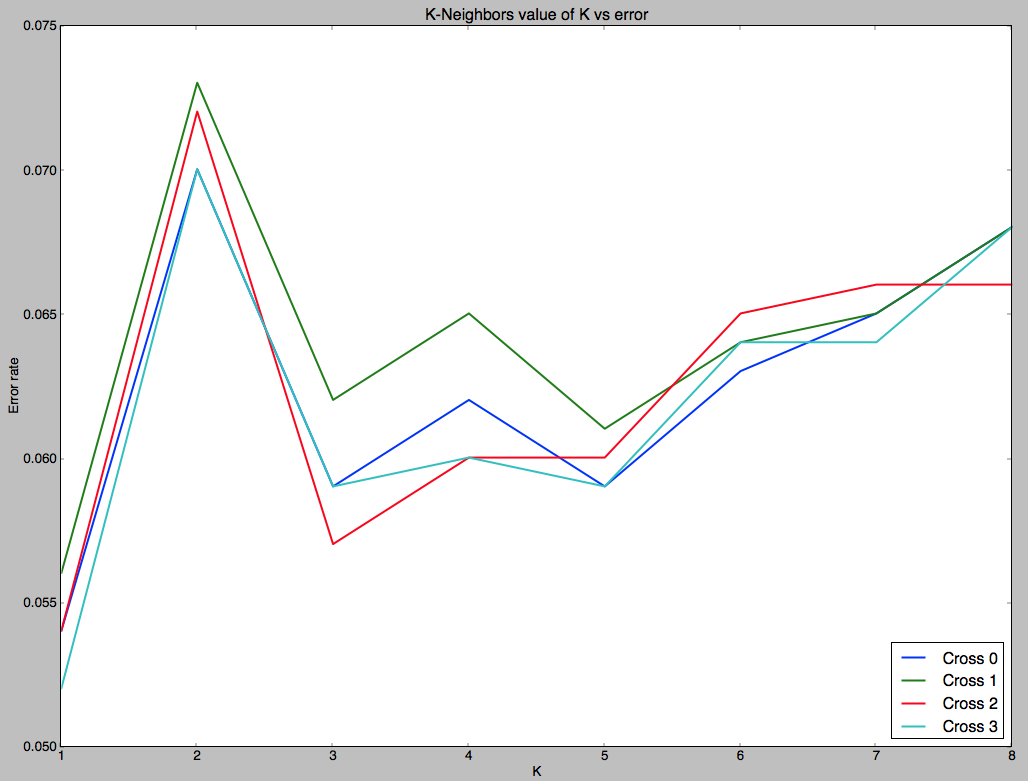
\includegraphics[width=0.9\textwidth]{figures/KN_kvalue}
	\caption{K-Nearest Neighbors - K vs error}
	\label{fig:KN_kvalue}
\end{figure}
\subsection{Naural Network}
For an artifitial neural network method we use a perceptron with one hidden layer which uses softmax function
on the output layer. We are optimizing number of nodes in a hidden layer. The lowest error rate occured with a
hidden nodes count of aproximetly 1.5 times a number of attributes, so about 26. This optimal number varies 
as the training subset changes in cross-validation, but still is close to that number. In the figure \ref{fig:NN_hiddennodes} 
we can see an average of error rates for various hidden neurons count.
\begin{figure}[!tbh]
	\centering
	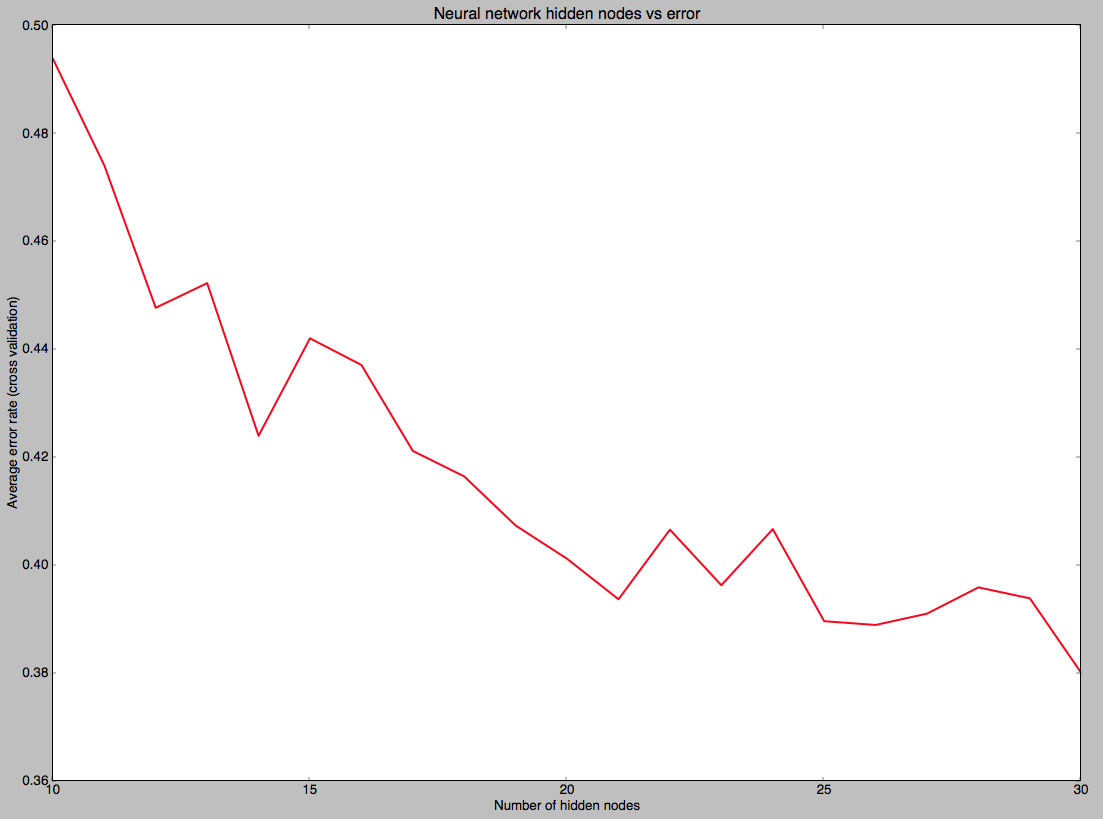
\includegraphics[width=0.9\textwidth]{figures/NN_hiddennodes}
	\caption{Neural Network - hidden nodes vs error}
	\label{fig:NN_hiddennodes}
\end{figure}
\subsection{Naive Bayes}
For Naive Bayes method we tried to estimate optimal features set (number of features), however no matter of what
classifier we used for feature selection using recursive feature elimination with cross-validation, the best accuracy was
obtained with selecting all features. In a plot (figure \ref{fig:NB_feature_selection}) we can see how accuracy of the method 
depends on number of features.
\begin{figure}[!tbh]
	\centering
	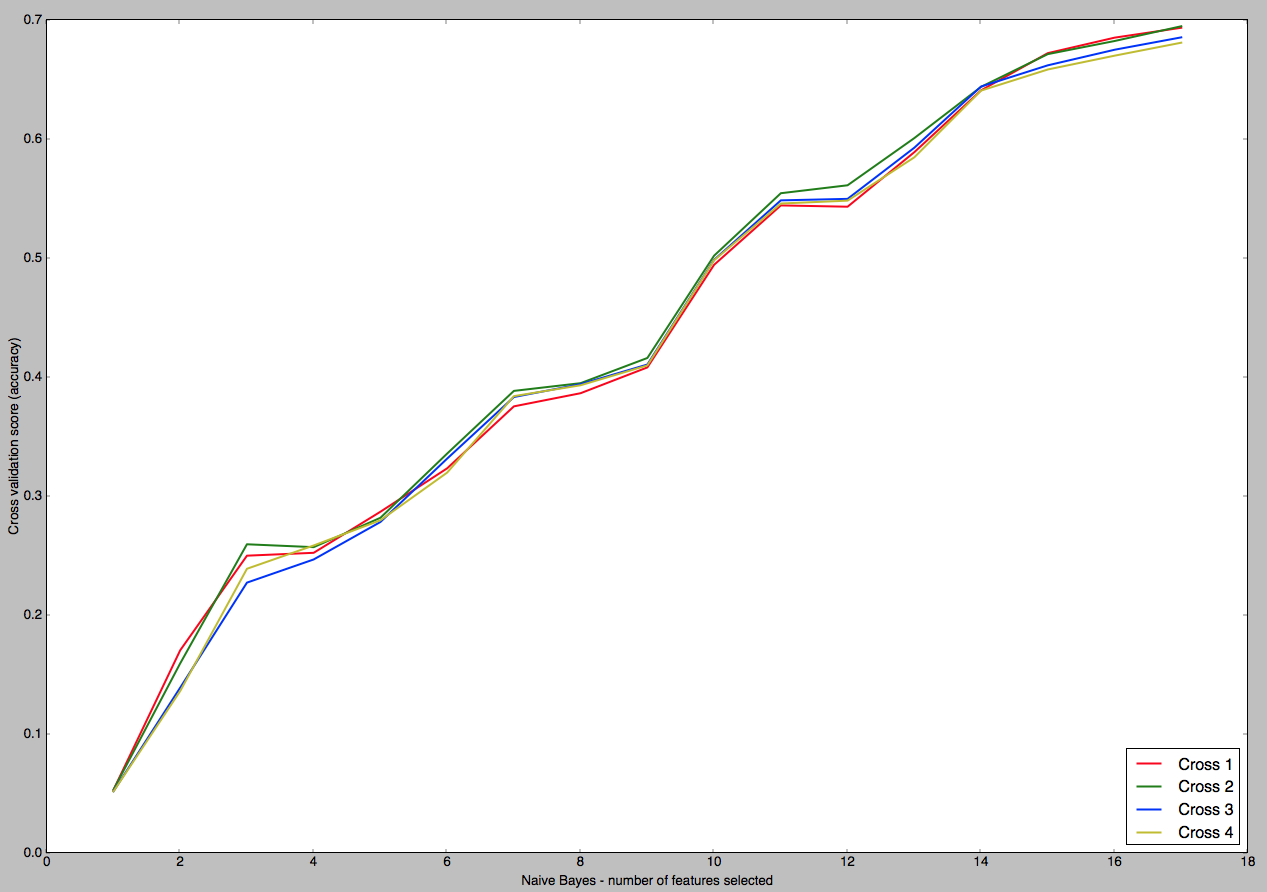
\includegraphics[width=0.9\textwidth]{figures/NB_feature_selection}
	\caption{Naive Bayes - features vs accuracy}
	\label{fig:NB_feature_selection}
\end{figure}
\section{Results}
For all methods, the error rate of predicting a letter basing of its attributes is below 50\%, what is quite a good result for
such a problem. The best results we got using K-Nearest Neighbors algorithm which with euclidesian mertic obtained less
than 5\% of bad answers. Out error rate is calculated as: \\
error\_rate = (predicted\_letters != actual\_letters) / number\_of\_tests

\begin{figure}[!t]
	\centering
	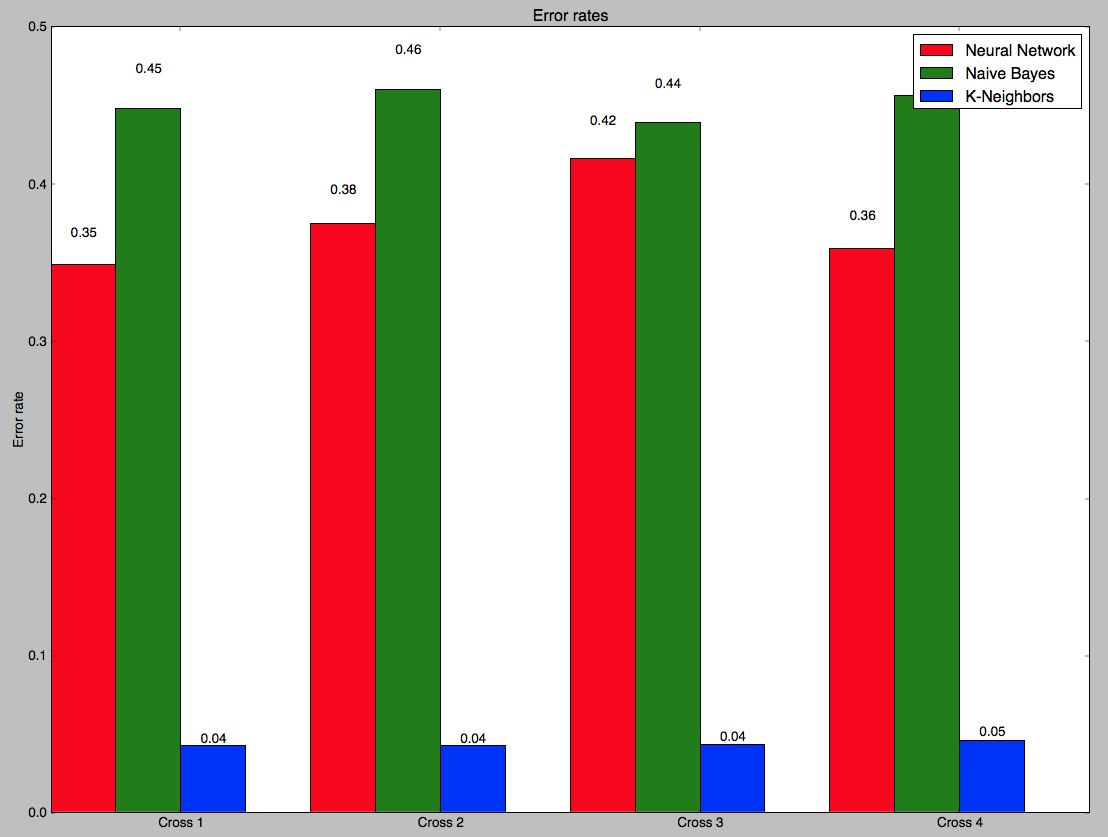
\includegraphics[width=0.85\textwidth]{figures/performance}
	\caption{Performance of methods in outer cross-validation loop}
	\label{fig:performance}
\end{figure} 
\begin{figure}[!t]
	\centering
	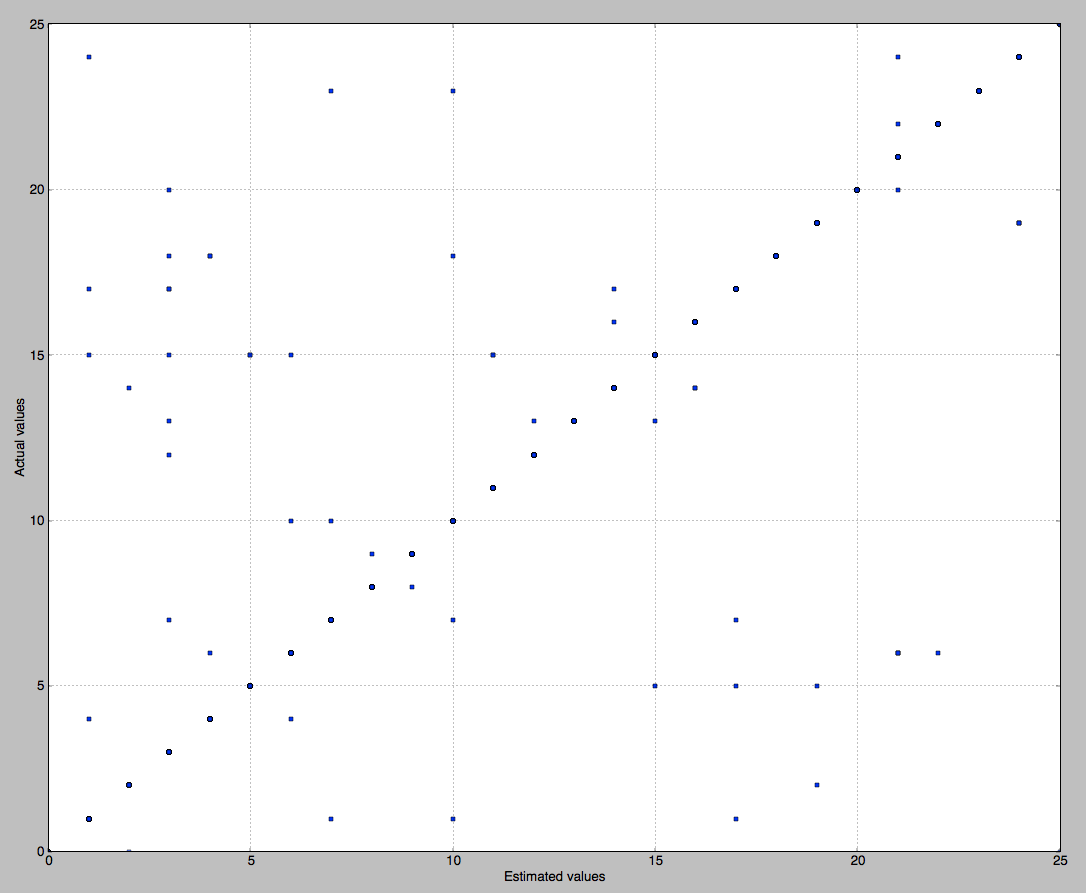
\includegraphics[width=0.85\textwidth]{figures/predictions}
	\caption{Predicted values vs actual values (KNN)}
	\label{fig:predictions}
\end{figure}
Below (figure \ref{fig:predictions}) we can see a plot describing how good letters are predicted by KNN method. 
From 5000 points used only a few are away from $x=y$ line. Most of the points are on that line, which means that
letters are predicted correctly. \\

Moreover, fitting our methods for all of the data (20000 records) we obtained on average 4\% of an error rate for KNN and 35\%, 44\% 
for Neural Network and Naive Bayes accordingly. We used K-fold cross-validation using all that data which forced us to use parallelism
computing every fold in a separate thread. 
\section{Comparison}
The boxplot below (figure \ref{fig:cross_errors}) shows that there are great differences between a performance of used methods. 
\begin{figure}[!tbh]
	\centering
	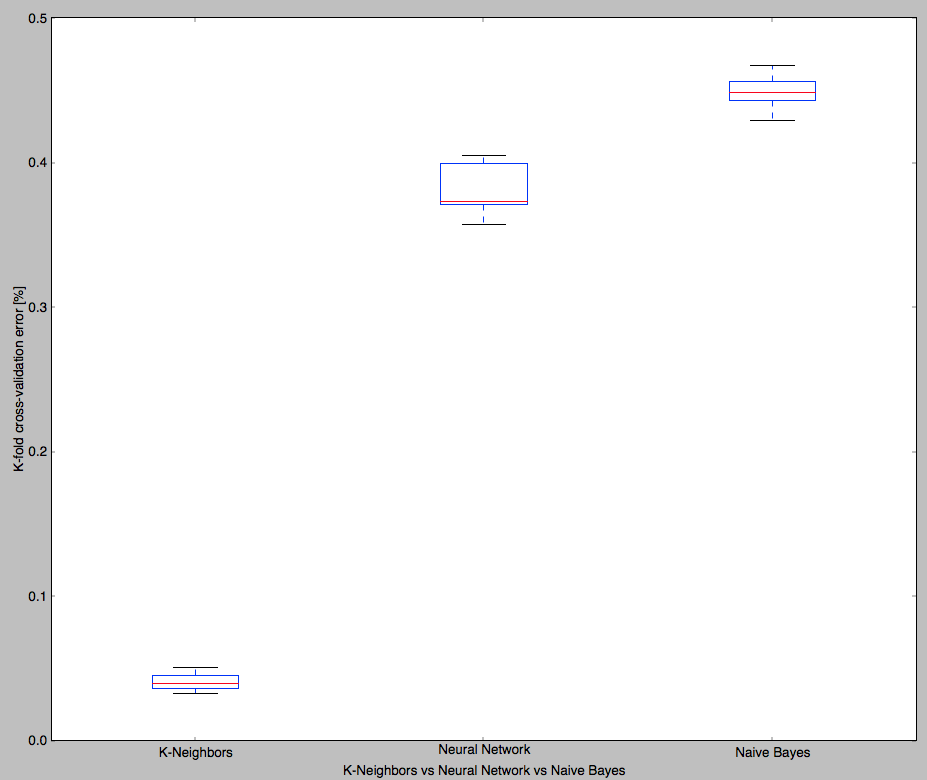
\includegraphics[width=0.9\textwidth]{figures/cross_errors}
	\caption{Cross-validation errors for all methods}
	\label{fig:cross_errors}
\end{figure}
We used also a paired t-test to compare selected methods with each other and additionally with a fake predictor, which 
classifies all outputs to be the largest class in the training data: \\
\begin{tabular}{l*{4}{c}r}
Compared alg. & t-test value & p-value & significantly \\
ANN vs Naive Bayes & -10.3 & 0.0 & True \\
ANN vs KNN & 57.8 & 0.0 & True \\
Naive Bayes vs KNN & 100.5 & 0.0 & True \\
Biggest Class vs ANN & -100.4 & 0.0 & True \\
Biggest Class vs KNN & -380.7 & 0.0 & True \\
Biggest Class vs Naive Bayes & -133.3 & 0.0 & True \\
\end{tabular} \\
The results shows us that all of the methods are significantly different in case of performance.
\section{Related work}
This dataset was used for letter recognition (classification) using Holland-style Adaptive Classifiers. The article is available on the following link: \\
\url{http://download.springer.com/static/pdf/733/art%253A10.1007%252FBF00114162.pdf?auth66=1414859976_6267eff4e2e0779ac8c3bd5c7c57b61c&ext=.pdf} 
The percentage of correct identifications they achieved varies between 50\% to 80\% depending on the settings, where the highest score is
obtained with the most computationally demanding settings. Refering to that article we can assume that our results are successful. 





